\documentclass[english,onecolumn]{scrartcl}
\usepackage[T1]{fontenc}
\usepackage{listings}
\usepackage{hyperref}
\usepackage{tabularx}
\usepackage{array}
\usepackage{booktabs}
\usepackage{multirow}
\usepackage{tikz-timing}
\usepackage{graphicx}
\usepackage{pdfpages}
\usepackage[style=ieee, backend=biber]{biblatex}

\definecolor{darkgreen}{HTML}{008000}
\lstset{frame=single,
    language=Haskell,
    breaklines=true,
    showspaces=false,
    showstringspaces=false,
    showtabs=false,
    basicstyle=\footnotesize,
    commentstyle=\color{darkgreen},
    keywordstyle=\color{blue},
    stringstyle=\color{purple},
    title=\lstname}
\def\tabularxcolumn#1{m{#1}}
\pagenumbering{roman}
\tikzset{timing/draw grid}
\addbibresource{references.bib}


\begin{document}
\title{ECE4095 Final Report}
\subtitle{H2V --- a Haskell to Verilog Compiler}
\author{Reuben D'Netto (22096620)}

\maketitle
\tableofcontents{}
\pagebreak{}
\pagenumbering{arabic}


\section{Significant Contributions}
\begin{itemize}
    \item Designed and implemented a Haskell to Verilog compiler
    \item Designed and implemented support for the following functions through a combination of generated and hard-coded Verilog:
        \begin{itemize}
            \item List operators: cons (:), concat (++)
            \item Higher order list functions: map, fold/reduce, zipWith
        \end{itemize}
    \item Designed and implemented support for N-degree parallel computation of lists, as defined by user
    \item Designed and implemented support for evaluation of higher order functions at compile-time
    \item Designed and implemented data flow graph generation
    \item Verified hardware generated for test cases using SignalTap
\end{itemize}

% Include poster such that it appears in the TOC without adding a heading to the page
% Code taken from: http://tex.stackexchange.com/questions/68272/make-section-headings-invisible
\newcommand\invisiblesection[1]{%
    \refstepcounter{section}%
    \addcontentsline{toc}{section}{\protect\numberline{\thesection}#1}%
    \sectionmark{#1}}

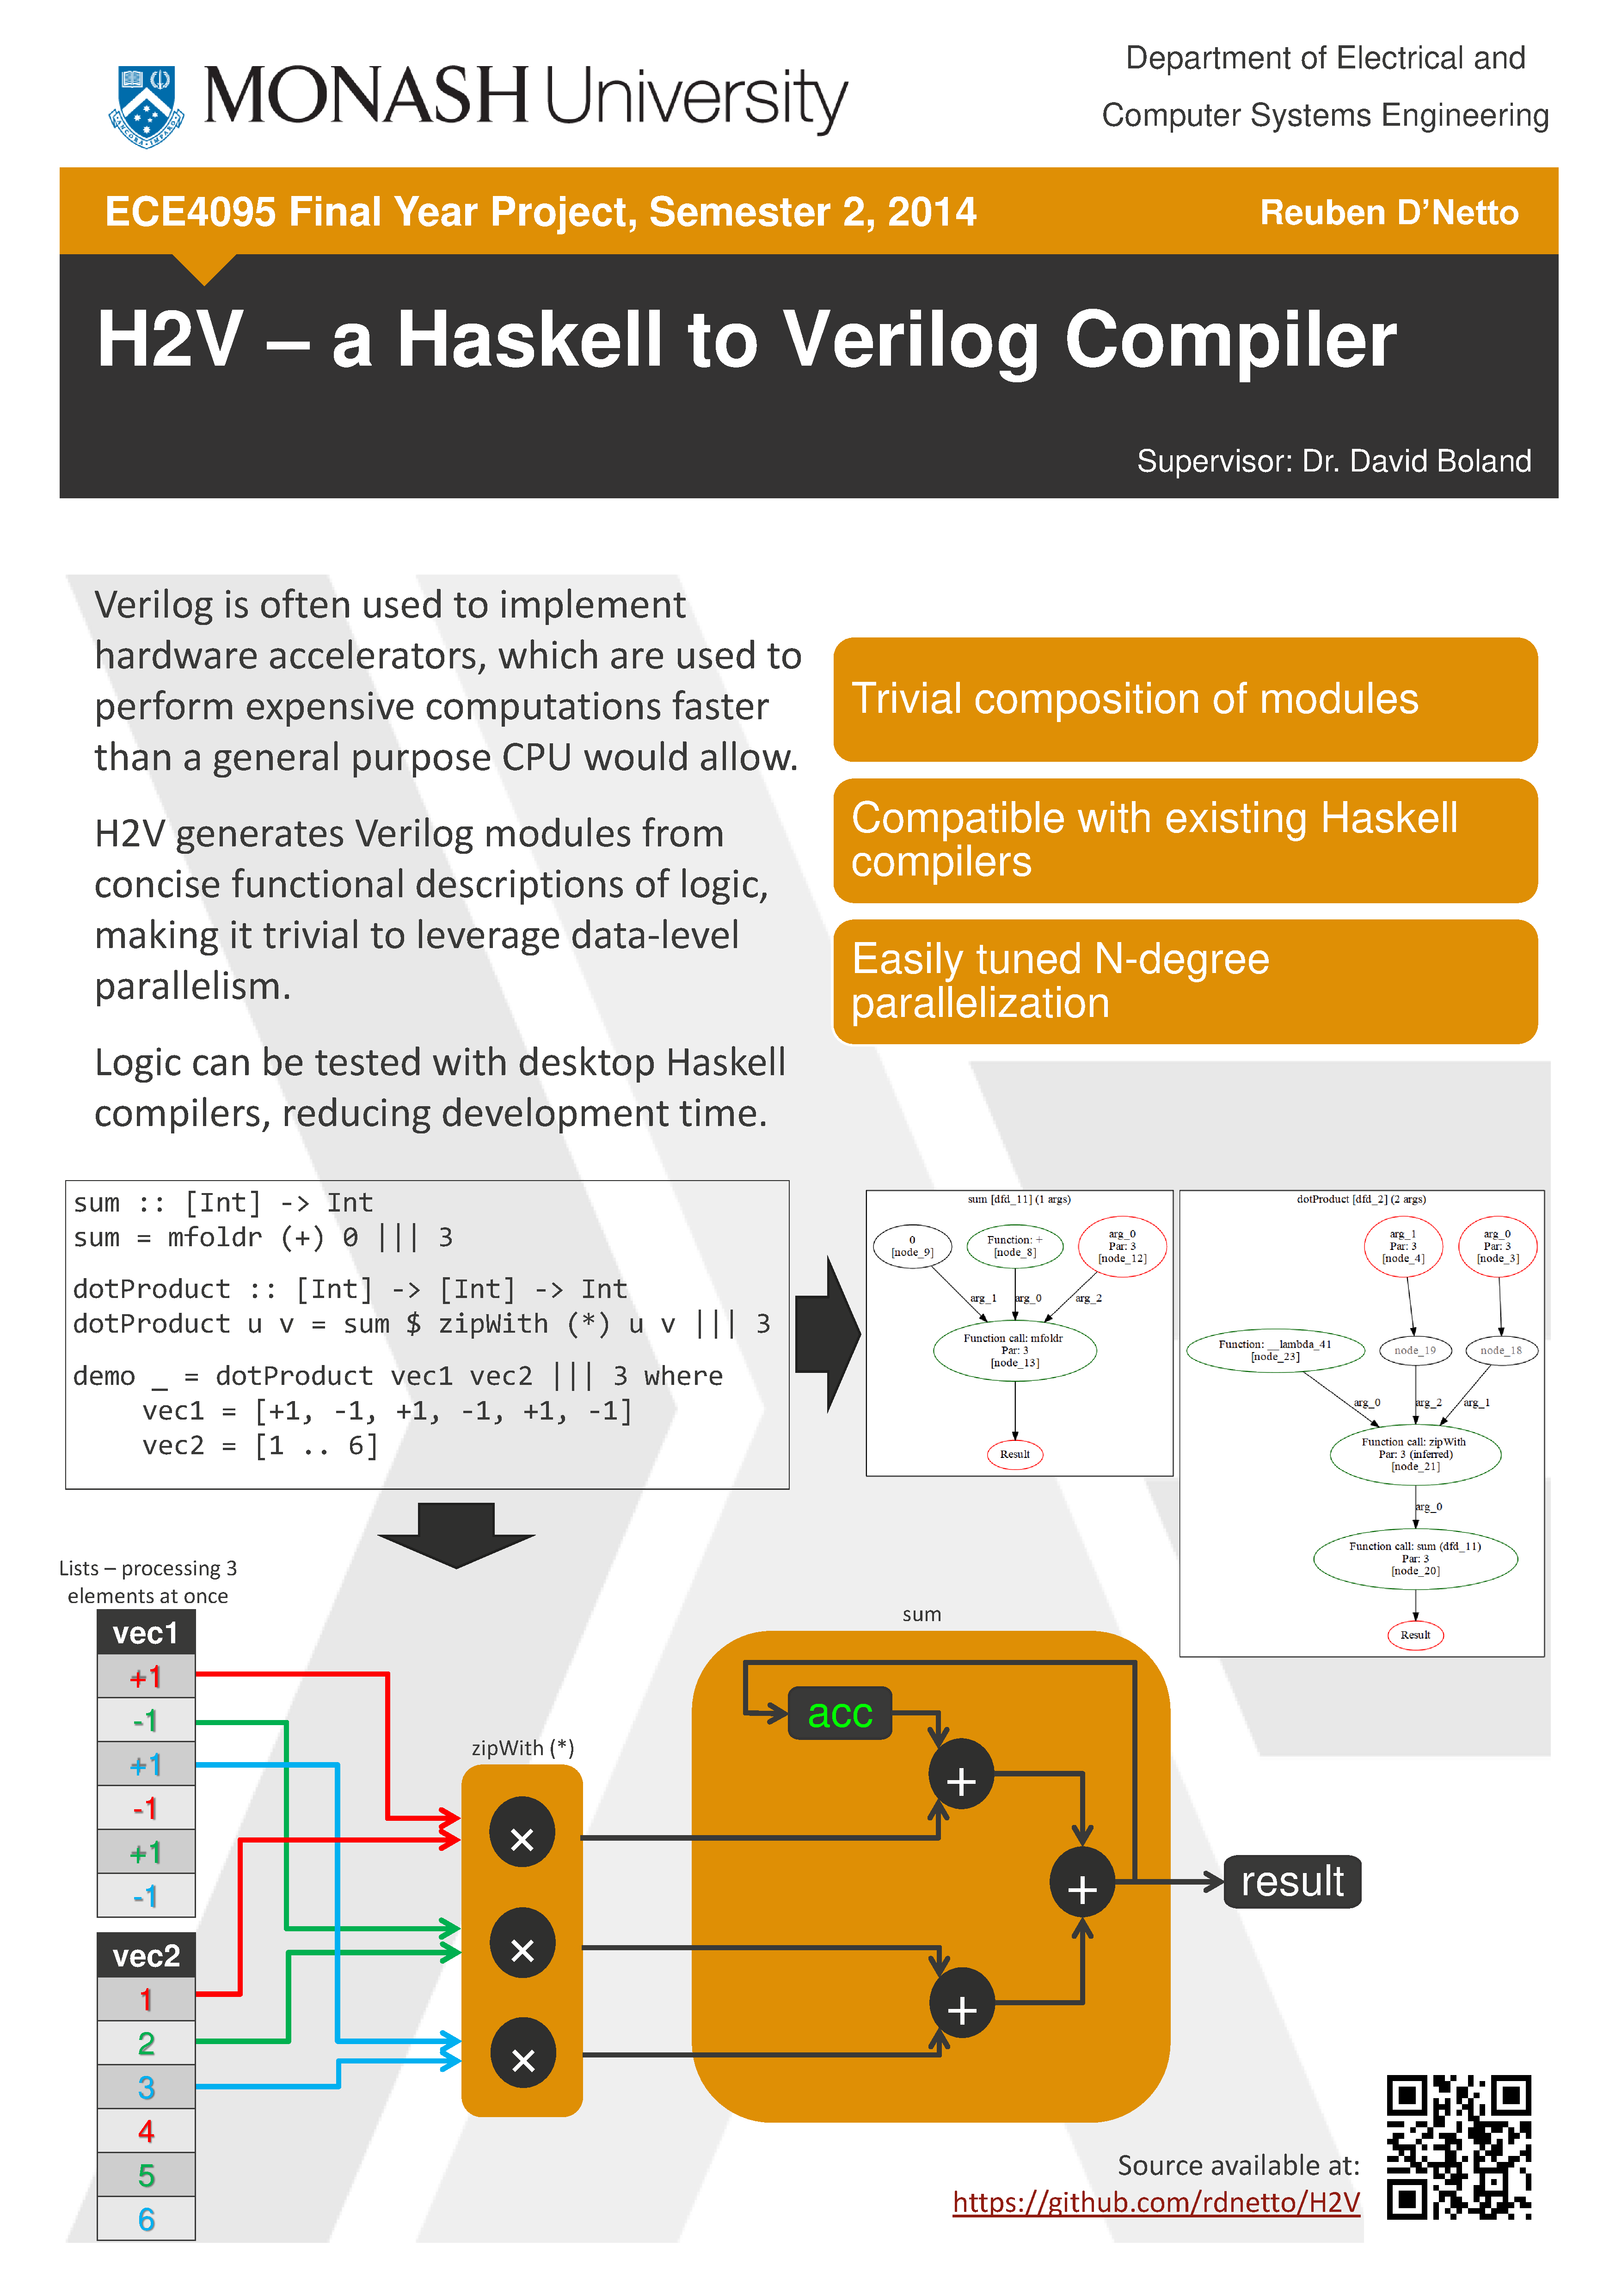
\includepdf[pages={1}, pagecommand={\invisiblesection{Poster}}]{../Poster/Poster.pdf}


\section{Summary}
% TODO: do this last
% what I did, how I did it, and why the results matter
% state topic and aim
% outline major stages
% summarise major results/outcomes and their significance

\section{Introduction}
% TODO: context, motivation/rationale, problem definition, aims/goals, scope, outline report structure

\subsection{Context \& Rationale}
Verilog is a commonly used hardware description language used for programming field programmable gate arrays (FPGAs).
Its uses may be broadly grouped into two categories: interfacing with low-level hardware, and accelerating computations which
would otherwise be performed sequentially on a microprocessor. Due to its low-level nature (which is necessary for the first class
of use cases), implementing computations directly in Verilog is extremely time consuming, and often complex as a result of the
parallelism that it enables.

H2V is a Haskell to Verilog compiler. Programs can be defined extremely consisely and simply in Haskell, and then compiled into an
appropriate set of Verilog modules. Since H2V is compatible with a subset of the Haskell standard, the same program code can be
compiled and tested using existing tools, facilitating faster and more thorough testing.

\subsection{Haskell}
Haskell is a strongly typed pure functional language with lazy evaluation, in contrast to C, which is a weakly typed imperative
language with strict evaluation. This means that all variables in Haskell are immutable, and all functions are unable to access,
modify, or preserve any state. These features make it ideal for use in parallel computations, where state translates directly to
bottlenecks.%
\footnote{In fact, these features overlap considerably with the recommendations in many C to hardware tools.\cite{C2H_UG}}
Furthermore, because Haskell programs are defined in terms of the expressions assigned to variables (instead of the instructions
to be evaluated by a microprocessor), H2V has a much cleaner and more direct mapping between expressions and hardware modules than
C-based tools have.


\subsection{Project Definition}
The goal of this project is to demonstrate the viability of a Haskell to Verilog compiler, and its advantages over similar tools
which compile imperative programs (e.g.\ in C) to hardware. A Haskell to Verilog compiler (H2V) was implemented, but as a proof of
concept rather than a completed tool. H2V supports only a subset of the Haskell 2010 standard and the associated standard
libraries.


\section{Literature Review}
% current state of field
% define the gap satisfied by my project
% justify trade offs for rejection of superior approaches
% TODO

%-C2H
%-why C2H is inferior - expand on this using the notes from the last meeting with David
%-existing functional approaches
Lorem ipsum blah blah blah


\section{Supported Features}
\subsection{Comparison to Requirements Analysis}
\begin{tabularx}{\textwidth}{l c X c}
\toprule
ID      & Type              & Description                 & Implemented
\\ \midrule

3.1.1a  & Requirement & Support a subset of Haskell 2010. & Yes
\\ \midrule

3.1.1b  & Requirement & Support tail-recursive functions. & Yes
\\ \midrule

3.1.2.1 & Optional    & Retain compatibility with existing Haskell compilers. & Yes
\\ \midrule

3.1.2.2 & Optional    & Support first class functions. & Yes
\\ \midrule

3.1.2.3 & Optional    & Support unary non-tail recursive functions with bijective mappings for arguments. & No
\\ \midrule

3.1.2.4 & Optional    & Support for compiling multiple files at once. & No
\\ \midrule

3.1.2.5 & Optional    & Loop vectorization of recursive functions. & No
\\ \midrule

3.1.2.6 & Optional    & Restructing of expressiong trees to reduce critical path. & No
\\ \midrule

3.1.2.7 & Optional    & Partial type inference. & Yes%
\footnote{Limited type inference is supported for scalar and list types. Type inference for higher order types is not supported.}
\\ \midrule

3.2.1   & Requirement & QSys Integration --- generation of C headers and component definitions. & No%
\footnote{See s\ref{sec:reqQsys}.}
\\ \midrule

3.2.2.1 & Optional    & Use optional features in Avalon bus protocol to improve performance. & N/A
\\ \midrule

3.2.2.2 & Optional    & Support Avalon Streaming interfaces. & No
\\ \midrule

3.3.1   & Requirement & Support for sequential reads from RAM. & Implicit%
\footnote{See s\ref{sec:reqDMA}.}
\\ \midrule

3.3.2   & Optional    & Support for sequential writes to RAM. & Implicit%
\footnote{See s\ref{sec:reqDMA}.}
\\ \midrule

3.3.3   & Optional    & Support for non-sequential reads from RAM. & No
\\ \midrule

3.3.4   & Optional    & Support for caching subsequent accesses. & N/A
\\ \midrule

%TODO: it would be a really good idea to implement this for at least the demo case
3.4.1.1 & Requirement & Results shall include benchmarks comparing H2V and C2H. & No
\\ \midrule

%TODO: update this cross-reference
3.4.1.2 & Requirement & The execution time of H2V accelerators shall be equal or better to those of C2H. & Yes%
\footnote{H2V is significantly faster than C2H in list-based benchmarks due to its support for parallelism. (refer to s FOO.)}
\\ \midrule

3.5.1   & Requirement & H2V shall be published under a free software license. & Yes%
\footnote{H2V is available at \url{https://github.com/rdnetto/H2V} under the GNU General Public License version 2 (GPLv2).}
\\ \bottomrule
\end{tabularx}


\subsubsection{QSys Integration}
\label{sec:reqQsys}
QSys integration was abandoned as the goal of the project shifted from implementing a finished tool (a task that would likely take
years) to demonstrating the viability of the concept. QSys integration is trivial to implement, to the extent that it could easily
be performed by hand. Consequently, this would have added little to the project.

A second factor in abandoning QSys integration was that it relied on the inherent assumption that the main application of H2V was
augmenting Nios soft-processors. This proved to be false, as accessing data stored in the processor's RAM would be limited to two
words per cycle in most cases (due to the constraints of the hardware). In contrast, H2V achieves optimal performance in
applications where it can read several words in the same clock cycle. There would therefore be little point in implementing QSys
integration, as it would be advantageous only in situations where the Avalon bus was not memory-mapped.%
\footnote{The Avalon-MM bus has a maximum bandwidth of 128 bytes per clock cycle,\cite[3-4]{C2H_AvalonSpec} and so could be connected
    to H2V modules without a significant reduction in throughput.}


\subsubsection{Direct Memory Access}
\label{sec:reqDMA}
Instead of implementing direct memory access, a well-defined list interface protocol was implemented. This has the advantage of
enabling parallelism beyond what the memory would support, as well as offering increased flexibility in allowing a variety of data
sources and sinks to be used. Since all related use cases in the requirements analysis have been satisfied, this requirement can
be regarded as completed.


\subsection{Supported Features}
% discuss exactly what is supported here
% this is also a good place to discuss the overall design of the compiler


\section{Future Work}
% TODO
% -parallelism inference
% -closures
% -full support for list functions

Blah\footnote{More blah}


\section{Conclusions}
% relate content to project aims
% summarise major findings
% highlight contributions of work
% acknowledge limitations
% make recommendations - further work, improvements


\pagebreak{}
\appendix
\section{Appendix --- Test Cases}
\subsection{Language Features}
\lstinputlisting{../../H2V/tests/f0.hs}
\lstinputlisting{../../H2V/tests/f1.hs}
\lstinputlisting{../../H2V/tests/guards.hs}
\lstinputlisting{../../H2V/tests/pattern_match.hs}
\lstinputlisting{../../H2V/tests/fib.hs}

\subsection{Higher Order Functions}
\lstinputlisting{../../H2V/tests/ho_arg.hs}
\lstinputlisting{../../H2V/tests/ho_flip.hs}
\lstinputlisting{../../H2V/tests/ho_pa.hs}
\lstinputlisting{../../H2V/tests/ho_return.hs}

\subsection{Lists}
\lstinputlisting{../../H2V/tests/lists.hs}
\lstinputlisting{../../H2V/tests/lists2.hs}
\lstinputlisting{../../H2V/tests/demo.hs}

\section{Appendix --- Source Code}
The source code is also available at \url{https://github.com/rdnetto/H2V}.

\lstinputlisting{../../H2V/main.hs}
\lstinputlisting{../../H2V/Common.hs}
\lstinputlisting{../../H2V/DfdDef.hs}
\lstinputlisting{../../H2V/GenerateDFD.hs}
\lstinputlisting{../../H2V/RenderGraphviz.hs}
\lstinputlisting{../../H2V/RenderVerilog.hs}
\lstinputlisting{../../H2V/AST_Display.hs}

\section{Appendix --- Include Files for H2V Programs}
\lstinputlisting{../../H2V/include/hs/H2V_Compat.hs}
\lstinputlisting{../../H2V/include/v/include.v}

\printbibliography

\end{document}

